\documentclass[conference,a4paper]{IEEEtran}

\usepackage[utf8]{inputenc}
\usepackage[T1]{fontenc}
\usepackage[spanish]{babel}
\usepackage{graphicx}
\usepackage{amsmath}
\usepackage{booktabs}
\usepackage{url}
\usepackage{float}
\usepackage{tikz}
\usetikzlibrary{arrows.meta, positioning, shadows.blur, fit, babel}
\usepackage{standalone}
\usepackage{placeins}
\usepackage{afterpage}
\usepackage{stfloats}
\usepackage{cuted}
\usepackage{caption}

\title{Clasificación y Reconstrucción de Objetos a partir de Perceptos Simulados de Prótesis Retinales}

\author{
\IEEEauthorblockN{Joel Jablonski}
\IEEEauthorblockA{
Universidad de San Andrés \\
Email: jjablonski@udesa.edu.ar}
\and
\IEEEauthorblockN{Estanislao Molina Abeniacar}
\IEEEauthorblockA{
Universidad de San Andrés \\
Email: emolinaabeniacar@udesa.edu.ar}
}

\begin{document}

\maketitle

\begin{abstract}
Las prótesis retinales buscan restaurar parcialmente la percepción visual mediante la estimulación eléctrica de la retina. Sin embargo, la información percibida por el usuario no corresponde a una imagen natural, sino a un percepto degradado, de baja resolución y dependiente de la geometría del implante. En este trabajo se estudia hasta qué punto dichos perceptos preservan información útil sobre objetos visuales. Para ello, se construyó un conjunto de datos a partir de máscaras de objetos de COCO, se generaron perceptos simulados mediante \textit{pulse2percept} para tres modelos de implante retinal y se evaluaron dos tareas: clasificación de objetos y reconstrucción de máscaras. En clasificación se compararon modelos KNN, CNN y CNN+GRU, incluyendo variantes de implante individual y fusión multi-implante. En reconstrucción se utilizaron arquitecturas tipo U-Net para recuperar la máscara binaria del objeto a partir del percepto. El mejor clasificador fue un KNN multi-implante, con accuracy de test de 0.611, superando a la arquitectura neuronal CNN+GRU, que obtuvo 0.575. Este resultado sugiere que, para el tamaño y características del conjunto de datos utilizado, una representación clásica basada en similitud directa y PCA puede ser más estable que una red neuronal entrenada desde cero. En reconstrucción, el mejor modelo fue una U-Net de fusión, con Dice de 0.9048 e IoU de 0.8756. Estos resultados sugieren que los perceptos simulados, aunque degradados, conservan información semántica y espacial que puede ser aprovechada por modelos de aprendizaje automático.
\end{abstract}

\begin{IEEEkeywords}
visión protésica, prótesis retinales, pulse2percept, clasificación de objetos, reconstrucción de imágenes, U-Net, CNN, KNN.
\end{IEEEkeywords}

\section{Introducción}

Las prótesis retinales constituyen una línea de investigación orientada a restaurar parcialmente la visión en personas con pérdida visual severa. A diferencia de una cámara convencional, estos dispositivos no transmiten una imagen completa y natural, sino que estimulan eléctricamente la retina mediante un arreglo limitado de electrodos. Como consecuencia, la percepción resultante suele ser degradada, de baja resolución, con pérdida de detalles y dependiente de la geometría del implante utilizado.

El objetivo inicial de este trabajo se relacionaba con una pregunta aplicada: ¿qué transformación o filtro podría aplicarse a una imagen para que una persona usuaria de una prótesis visual pueda interpretar mejor la escena? Esta pregunta tiene motivación práctica, ya que en visión protésica no necesariamente resulta óptimo mostrar la imagen original tal como fue capturada. Debido al ancho de banda limitado de los implantes y a la baja resolución perceptual, puede ser más útil simplificar la escena, resaltar objetos relevantes o transformar la imagen en una representación más interpretable. Esta idea se relaciona con trabajos previos en visión protésica simulada que proponen transformar la escena original en representaciones más esquemáticas y semánticamente relevantes, por ejemplo mediante segmentación de objetos, extracción de bordes estructurales o simplificación de escenas~\cite{han2021,sanchezgarcia2018}.

Sin embargo, evaluar directamente filtros visuales para usuarios reales o incluso para sujetos en experimentos psicofísicos requiere un diseño experimental más complejo, validación perceptual y métricas subjetivas de comprensión visual. Por ese motivo, en este trabajo se abordó una etapa previa: construir un banco de prueba objetivo para medir cuánta información semántica y espacial se conserva después de simular el pasaje de una imagen por distintos modelos de implantes retinales. 

La hipótesis de trabajo es que, si un percepto simulado conserva información útil sobre el objeto original, entonces un modelo computacional debería poder recuperar parte de esa información. Para evaluar esta hipótesis se definieron dos tareas complementarias. La primera es clasificación de objetos, donde el objetivo es predecir la clase del objeto a partir del percepto. Esta tarea mide la información semántica preservada. La segunda es reconstrucción de máscaras, donde el objetivo es recuperar la forma espacial del objeto. Esta tarea mide la información geométrica preservada.

De este modo, el trabajo no pretende resolver directamente el problema completo de visión protésica en usuarios reales, sino aportar una metodología intermedia para comparar representaciones, implantes y estrategias de preprocesamiento. En un desarrollo futuro, este mismo esquema podría utilizarse para evaluar filtros candidatos antes de realizar pruebas con usuarios: si un filtro genera perceptos que permiten mejor clasificación o reconstrucción, entonces podría considerarse una representación más informativa para una prótesis visual. La Fig.~\ref{fig:pipeline} resume este flujo general, desde la imagen y la máscara original hasta la generación de perceptos simulados y las dos tareas evaluadas.


\begin{figure*}[!t]
    \centering
    
\includegraphics[width=1\textwidth]{fig1.pdf}
    \caption{Esquema general del trabajo: a partir de objetos segmentados se generan perceptos simulados de prótesis retinales y se evalúa la información preservada mediante clasificación y reconstrucción.}
    \label{fig:pipeline}
\end{figure*}

\section{Conjunto de Datos}

El conjunto de datos se construyó a partir de COCO~\cite{coco}, un dataset ampliamente utilizado en visión por computadora que contiene imágenes de escenas naturales con anotaciones de objetos e instancias segmentadas. En este trabajo no se utilizaron las imágenes RGB completas como entrada principal, sino las máscaras binarias de objetos. Esta decisión simplifica el problema y permite concentrarse en la preservación de forma, ubicación y categoría del objeto.

Se seleccionaron cuatro clases de objetos: \textit{person}, \textit{car}, \textit{chair} y \textit{dining table}. Estas clases permiten trabajar con objetos de distinta complejidad geométrica: personas con extremidades y formas articuladas, autos con siluetas compactas, sillas con estructuras finas y mesas con variabilidad de forma.

El proceso de extracción consistió en decodificar las segmentaciones de COCO para obtener máscaras binarias. Luego, cada máscara fue redimensionada manteniendo su relación de aspecto y completada con padding negro hasta obtener una imagen cuadrada de $256 \times 256$ píxeles. Esta decisión evita deformar la geometría del objeto, lo cual es importante porque la forma de la máscara es parte central del problema. En la Fig.~\ref{fig:mascaras} se muestran ejemplos de las máscaras binarias utilizadas como punto de partida.

\begin{figure}[H]
    \centering
    % INSERTAR IMAGEN: ejemplos de máscaras extraídas por clase.
    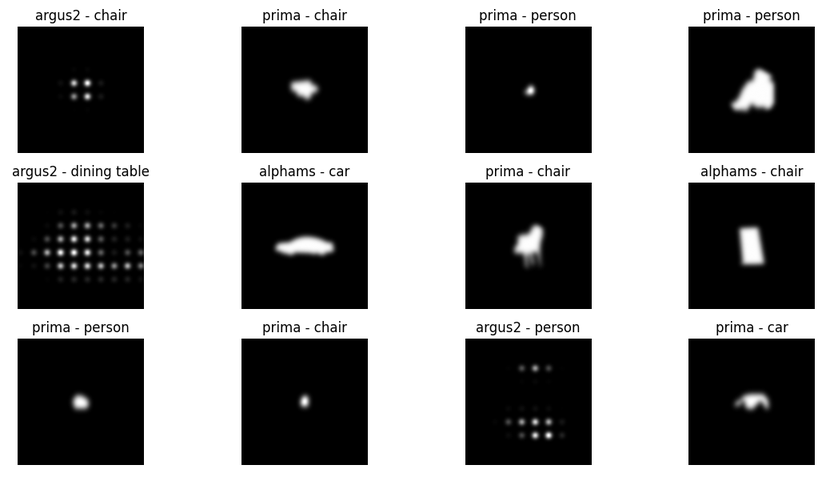
\includegraphics[width=1\linewidth]{figs/ejemplos_mascaras.png}
    \caption{Ejemplos de máscaras binarias extraídas desde COCO para las clases seleccionadas.}
    \label{fig:mascaras}
\end{figure}

A partir de las máscaras seleccionadas se generaron perceptos simulados para tres modelos de implante: Argus II, PRIMA y Alpha-AMS. Para cada muestra original se obtuvo un percepto por cada implante, por lo que una misma máscara produjo tres observaciones perceptuales distintas. Esto permite analizar tanto el desempeño por implante individual como el efecto de combinar información de múltiples implantes.

Para evitar data leakage entre entrenamiento, validación y prueba, la división del conjunto de datos se realizó por \textit{sample\_id} y no por fila individual. Esta decisión es fundamental porque cada objeto tiene varios perceptos asociados, uno por implante. Si la partición se hiciera fila por fila, el mismo objeto podría aparecer en entrenamiento con un implante y en test con otro, generando \textit{data leakage}. Por lo tanto, todos los perceptos de una misma muestra se asignaron al mismo split. El Cuadro~\ref{tab:dataset} resume las principales características del conjunto de datos utilizado.

\begin{table}[H]
\centering
\caption{Resumen del conjunto de datos utilizado.}
\label{tab:dataset}
\begin{tabular}{lc}
\toprule
Caracter\'{\i}stica & Valor \\
\midrule
Clases & person, car, chair, dining table \\
Tama\~no de m\'ascara & $256 \times 256$ \\
Implantes simulados & Argus II, PRIMA, Alpha-AMS \\
Perceptos por muestra & 3 \\
Tarea 1 & Clasificaci\'on de objeto \\
Tarea 2 & Reconstrucci\'on de m\'ascara \\
Distribuci\'on por clase & person: 900, car: 900, chair: 900, dining table: 624 \\
\bottomrule
\end{tabular}
\end{table}

\section{Generación de Perceptos Simulados}

La generación de perceptos se realizó con la librería \textit{pulse2percept}. En este trabajo, la librería se utilizó para transformar máscaras binarias de objetos en perceptos simulados de prótesis retinales. El flujo conceptual fue:

\begin{equation}
\text{máscara binaria} \rightarrow \text{estimulación del implante} \rightarrow \text{percepto simulado}.
\end{equation}

Primero, la máscara se convierte en un estímulo visual mediante \textit{ImageStimulus}. Luego, ese estímulo se redimensiona a la geometría del implante correspondiente. Esto es necesario porque cada implante posee una cantidad y disposición diferente de electrodos. Después, el estímulo redimensionado se asigna al implante, generando una matriz de activaciones por electrodo.

Es importante aclarar que la señal guardada no representa un tren temporal fisiológicamente completo de pulsos eléctricos. En este trabajo se utilizó como una matriz de intensidad o activación por electrodo. Esta simplificación permite construir un pipeline controlado de simulación y aprendizaje automático, aunque no modela todos los aspectos biofísicos de una prótesis real.

Finalmente, el modelo perceptual utilizado fue \textit{ScoreboardModel}, que proyecta la activación de los electrodos sobre una grilla espacial para obtener una imagen perceptual simulada. El percepto resultante se normaliza y se guarda como imagen en escala de grises. La Fig.~\ref{fig:perceptos_implante} muestra ejemplos de cómo una misma máscara puede producir perceptos distintos según el implante simulado.

\begin{figure}[H]
    \centering
    % INSERTAR IMAGEN: para una misma máscara, mostrar perceptos ArgusII, PRIMA y AlphaAMS.
    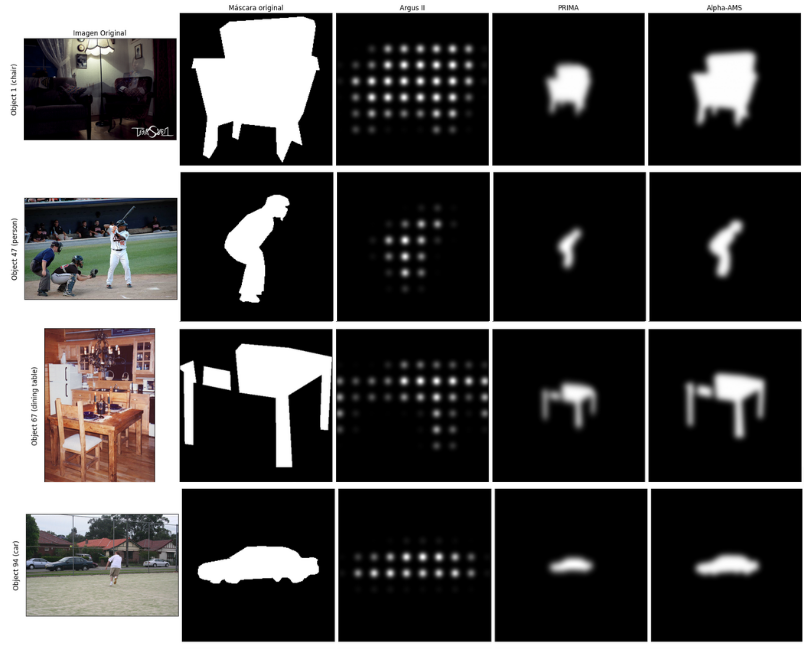
\includegraphics[width=1\linewidth]{figs/perceptos_por_implante.png}
    \caption{Ejemplo de perceptos simulados para una misma máscara usando distintos modelos de implante. Las imágenes se renderizan en una grilla de $256 \times 256$ píxeles para visualización, pero la información perceptual está limitada por la geometría del implante. En particular, Argus II posee 60 electrodos dispuestos aproximadamente en una grilla de $10 \times 6$, lo que ilustra la fuerte reducción de resolución respecto de la máscara original.}
    \label{fig:perceptos_implante}
\end{figure}

En sintesis, \textit{pulse2percept} no se utilizó para modelar la experiencia visual completa de un paciente, sino como una herramienta de simulación controlada para estudiar cómo distintas geometrías de implante degradan una misma representación visual.

\section{Métodos}

\subsection{Clasificación de objetos}

La primera tarea evaluada fue la clasificación de objetos a partir de perceptos. El objetivo fue estimar la clase del objeto original usando únicamente la información degradada contenida en el percepto.

Se evaluaron modelos clásicos y neuronales. Como baseline se utilizó KNN, tanto para perceptos de implante individual como para fusión multi-implante. En el caso de un solo implante, cada percepto se cargó en escala de grises, se redimensionó a $64 \times 64$, se normalizó al rango $[0,1]$ y se aplanó en un vector de 4096 características. Luego se aplicó un pipeline compuesto por estandarización, PCA y KNN:

\begin{equation}
\text{percepto} \rightarrow \text{flatten} \rightarrow \text{StandardScaler} \rightarrow \text{PCA} \rightarrow \text{KNN}.
\end{equation}

Para el modelo KNN multi-implante, se concatenaron los vectores correspondientes a Argus II, PRIMA y Alpha-AMS para un mismo \textit{sample\_id}. De esta manera, el clasificador recibe una representación más rica del objeto, formada por tres perceptos distintos de la misma máscara. Este modelo permite evaluar si la información de diferentes implantes es complementaria.

Además, se entrenaron modelos neuronales basados en CNN. La arquitectura CNN utiliza un encoder convolucional compuesto por cuatro bloques de convolución, normalización batch, ReLU y max pooling. Luego se aplica un \textit{Adaptive Average Pooling}, una capa lineal para obtener un embedding y una cabeza clasificadora con capas lineales y dropout. La salida son logits de clase entrenados con \textit{CrossEntropyLoss}.

Para fusionar información de múltiples implantes se utilizó una arquitectura CNN+GRU. En este caso, cada percepto de implante se procesa con el mismo encoder CNN para obtener una secuencia de embeddings. Luego, una GRU integra la información de los tres implantes y produce una representación final para clasificación. Esta arquitectura permite modelar la fusión multi-implante de forma aprendida, en lugar de realizar únicamente una concatenación fija de vectores. La Fig.~\ref{fig:clasificacion} esquematiza las dos arquitecturas neuronales de clasificación: el modelo de percepto individual y el modelo multi-implante con fusión mediante GRU. 

En términos de complejidad, la CNN individual utilizada para clasificación posee aproximadamente $4.3 \times 10^5$ parámetros entrenables, considerando \textit{feat\_dim}=128 y cuatro clases de salida. La arquitectura CNN+GRU posee aproximadamente $5.3 \times 10^5$ parámetros, ya que agrega una GRU de dimensión oculta 128 para fusionar los embeddings de los tres implantes.

\begin{figure}[H]
    \centering
    % INSERTAR IMAGEN: esquema de CNN y CNN+GRU.
    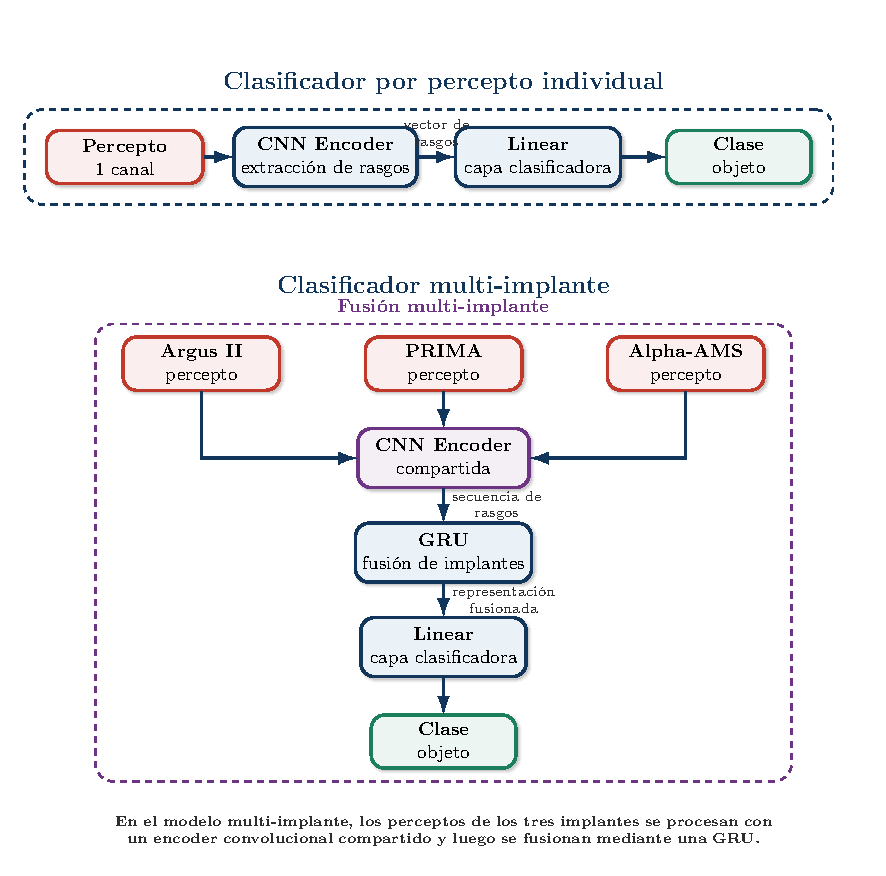
\includegraphics[width=1\linewidth]{figs/fig4.pdf}
    \caption{Arquitecturas utilizadas para clasificación: CNN de implante individual y CNN+GRU para fusión multi-implante.}
    \label{fig:clasificacion}
\end{figure}

\subsection{Reconstrucción de máscaras}

La segunda tarea fue la reconstrucción de máscaras binarias. A diferencia de la clasificación, donde la salida es una etiqueta discreta, en reconstrucción el modelo debe producir una imagen espacial. La tarea se define como:

\begin{equation}
\text{percepto} \rightarrow \text{máscara reconstruida}.
\end{equation}

Para esta tarea se utilizó una arquitectura tipo U-Net liviana. La elección de U-Net se debe a que es una arquitectura adecuada para problemas de segmentación y reconstrucción píxel a píxel, donde la salida conserva la estructura espacial de la entrada. La red posee un encoder que reduce progresivamente la resolución y extrae características globales, un bottleneck que concentra la representación más abstracta y un decoder que recupera la resolución espacial.

La arquitectura incluye conexiones de salto entre el encoder y el decoder. Estas conexiones permiten combinar información semántica profunda con detalles espaciales de mayor resolución. Esto es especialmente importante en este problema, porque los perceptos simulados son borrosos y de baja resolución, por lo que la reconstrucción de bordes y siluetas depende de conservar la mayor cantidad posible de información espacial.

Se entrenaron dos tipos de modelos. Primero, una U-Net individual para cada implante, con una entrada de un canal. Segundo, una U-Net de fusión multi-implante, donde los perceptos de Argus II, PRIMA y Alpha-AMS se apilan como canales de entrada. En todos los casos, la salida de la red es un canal de logits. Durante la evaluación se aplica una sigmoid y un umbral de 0.5 para obtener la máscara binaria final.

La función de pérdida utilizada fue una combinación de \textit{Binary Cross Entropy with Logits} y Dice Loss. Esta combinación es adecuada para segmentación binaria porque BCE penaliza errores píxel a píxel, mientras que Dice Loss favorece la superposición global entre la máscara predicha y la máscara objetivo. La arquitectura general de la U-Net utilizada para esta tarea se muestra en la Fig.~\ref{fig:unet}.


\begin{strip}
\centering
\vspace{-0.5em}
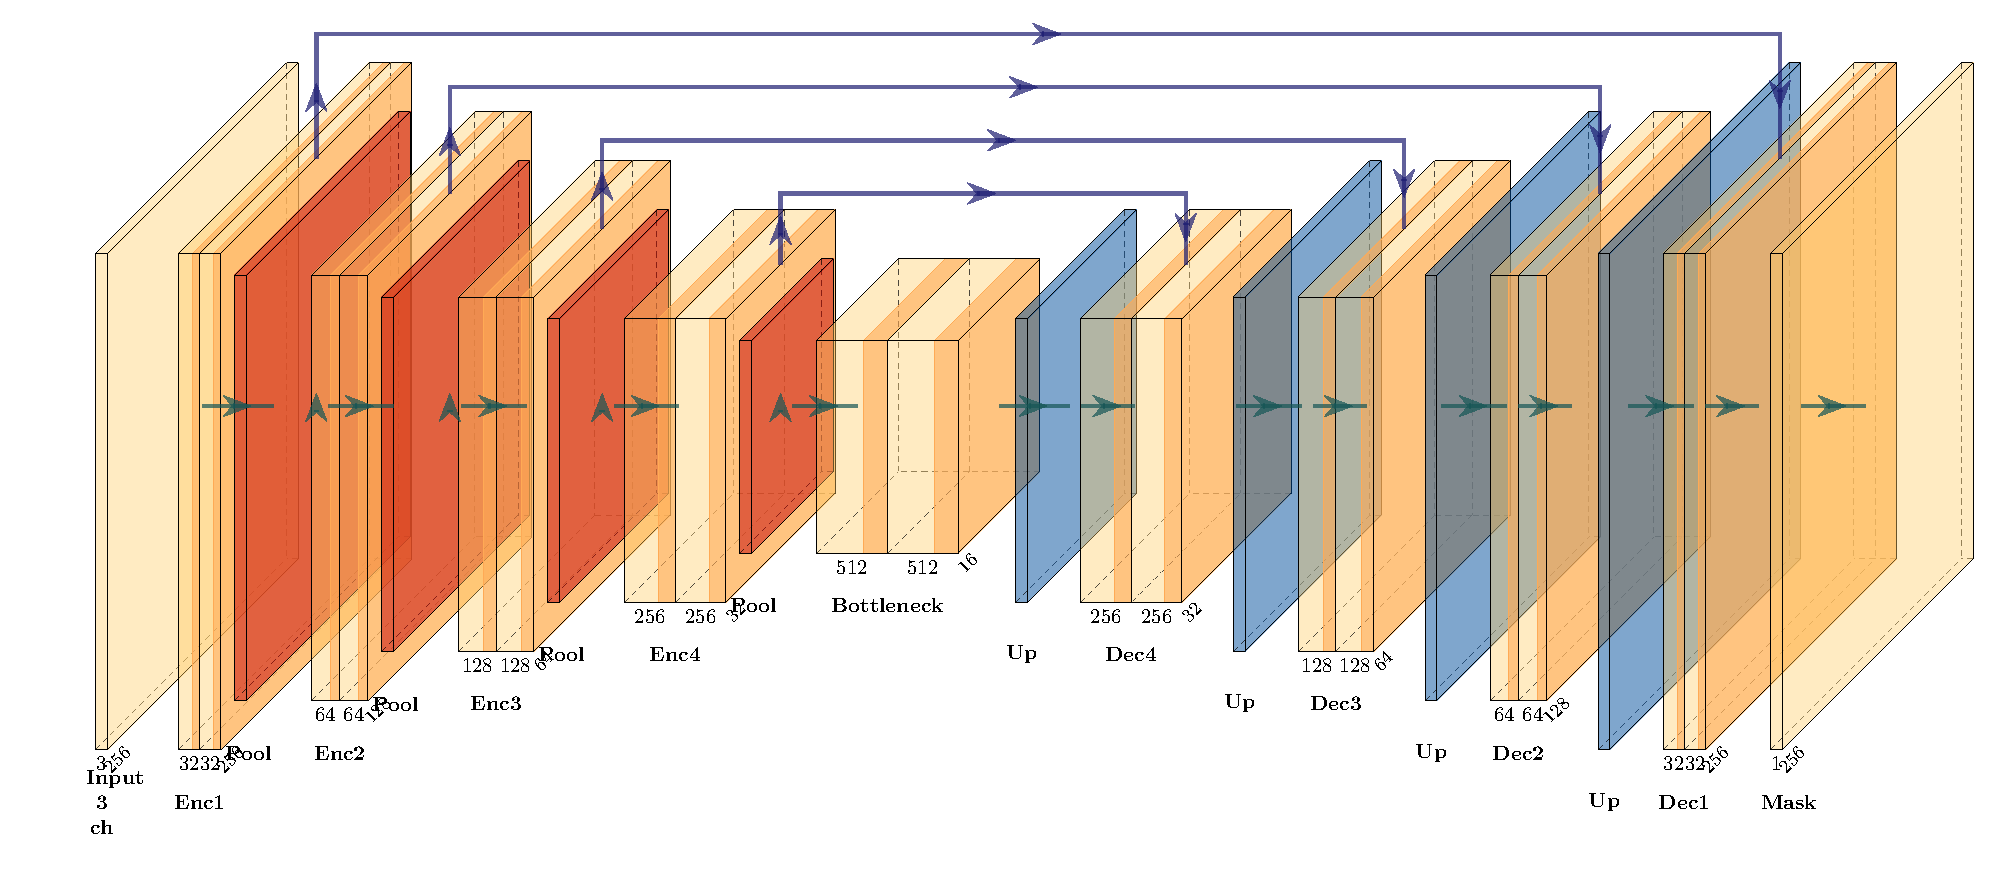
\includegraphics[width=\textwidth]{figs/arquitectura_unet.pdf}
\captionof{figure}{Arquitectura U-Net utilizada para reconstrucción de máscaras a partir de perceptos simulados.}
\label{fig:unet}
\vspace{-1em}
\end{strip}

La U-Net de reconstrucción es más grande que los clasificadores: con \textit{base\_channels}=32 posee aproximadamente $7.77 \times 10^6$ parámetros entrenables, tanto en la versión de implante individual como en la de fusión multi-implante. La diferencia entre ambas versiones es mínima, ya que solo cambia el número de canales de entrada de la primera convolución.

\section{Resultados}

\subsection{Resultados de clasificación}

El Cuadro~\ref{tab:clasificacion} resume los principales resultados de clasificación. El mejor modelo fue el KNN multi-implante, con una accuracy de test de 0.611. Esto indica que la combinación de perceptos provenientes de los tres implantes aporta información adicional respecto de usar implantes individuales. Como referencia, se incluye un baseline trivial que siempre predice la clase mayoritaria. Dado que la distribución final contiene 900 muestras para \textit{person}, \textit{car} y \textit{chair}, y 624 para \textit{dining table}, este baseline alcanza una accuracy aproximada de 0.271.

\begin{table}[H]
\centering
\caption{Resultados de clasificación en test.}
\label{tab:clasificacion}
\begin{tabular}{lc}
\toprule
Modelo & Accuracy test \\
\midrule
Baseline mayoría & 0.271 \\
KNN Argus II & 0.561 \\
KNN PRIMA & 0.571 \\
KNN Alpha-AMS & 0.567 \\
KNN multi-implante & \textbf{0.611} \\
CNN Argus II & 0.509 \\
CNN PRIMA & 0.563 \\
CNN Alpha-AMS & 0.561 \\
CNN+GRU & 0.575 \\
\bottomrule
\end{tabular}
\end{table}

La CNN+GRU fue el mejor modelo neuronal, con accuracy de test de 0.575. Si bien superó a las CNN individuales, no alcanzó el rendimiento del KNN multi-implante. Esto sugiere que, para el tamaño y características del conjunto de datos utilizado, una representación clásica basada en PCA y KNN resultó más estable que una red neuronal entrenada desde cero.

En el mejor modelo, las clases \textit{car}, \textit{person} y \textit{dining table} fueron reconocidas con mejor desempeño relativo, mientras que \textit{chair} resultó ser la clase más difícil. Esto puede deberse a que las sillas poseen estructuras delgadas, huecos y mayor variabilidad geométrica, características que pueden perderse con mayor facilidad en perceptos degradados. La matriz de confusión de la Fig.~\ref{fig:confusion_knn} permite observar con más detalle estos patrones de error, especialmente las confusiones asociadas a la clase \textit{chair}.

\begin{figure}[H]
    \centering
    % INSERTAR IMAGEN: matriz de confusión del KNN multi-implante.
    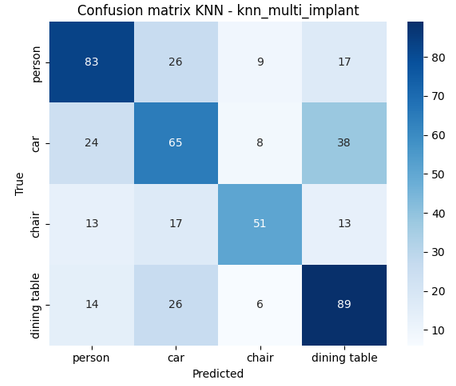
\includegraphics[width=1\linewidth]{figs/confusion_knn_multi.png}
    \caption{Matriz de confusión del mejor clasificador: KNN multi-implante.}
    \label{fig:confusion_knn}
\end{figure}

\subsection{Resultados de reconstrucción}

Los resultados de reconstrucción fueron evaluados mediante Dice, IoU y pixel accuracy. Dice e IoU son las métricas principales, ya que miden la superposición entre la máscara predicha y la máscara real. La pixel accuracy también se reporta, aunque debe interpretarse con cuidado porque en segmentación binaria gran parte de la imagen puede corresponder al fondo. El Cuadro~\ref{tab:reconstruccion} presenta la comparación cuantitativa entre los modelos de reconstrucción entrenados.

\begin{table}[H]
\centering
\caption{Resultados de reconstrucción de máscaras en test.}
\label{tab:reconstruccion}
\begin{tabular}{lccc}
\toprule
Modelo & Dice & IoU & Pixel acc. \\
\midrule
U-Net Argus II & 0.8829 & 0.8351 & 0.9856 \\
U-Net PRIMA & 0.8711 & 0.8246 & 0.9817 \\
U-Net Alpha-AMS & 0.9019 & 0.8623 & 0.9863 \\
U-Net fusión & \textbf{0.9048} & \textbf{0.8756} & \textbf{0.9891} \\
\bottomrule
\end{tabular}
\end{table}

El mejor modelo fue la U-Net de fusión multi-implante, con Dice de 0.9048, IoU de 0.8756 y pixel accuracy de 0.9891. El segundo mejor modelo fue la U-Net basada en Alpha-AMS, lo que indica que este implante individual ya generaba perceptos altamente informativos para la tarea de reconstrucción. Aun así, la fusión multi-implante logró el mejor resultado global.

Las curvas de entrenamiento y validación de la U-Net de fusión se muestran en la Fig.~\ref{fig:curvas_recon}. Allí se observa una disminución progresiva de la pérdida y un aumento de las métricas Dice e IoU durante el entrenamiento, con cierta variabilidad en validación esperable para el tamaño del conjunto de datos.

Cualitativamente, las reconstrucciones de la Fig.~\ref{fig:reconstrucciones} muestran que el modelo recupera correctamente la silueta general de los objetos. Las limitaciones aparecen principalmente en bordes irregulares, partes delgadas, huecos internos y componentes pequeños separados del cuerpo principal. Esto es consistente con la degradación introducida por la simulación perceptual: la red no reconstruye una copia exacta de la máscara original, sino una versión plausible y suavizada a partir de información incompleta.

\begin{strip}
\centering
\vspace{-0.5em}
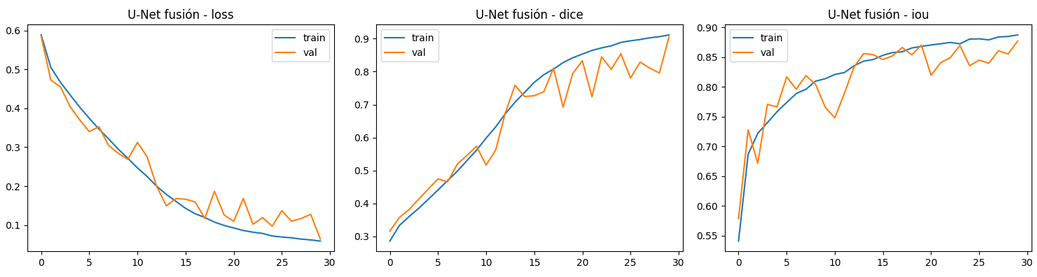
\includegraphics[width=1\textwidth]{figs/curvas_unet_fusion.png}
\captionof{figure}{Curvas de entrenamiento y validación para el modelo de reconstrucción.}
\label{fig:curvas_recon}
\vspace{-1em}
\end{strip}

\begin{figure}[!t]
    \centering
    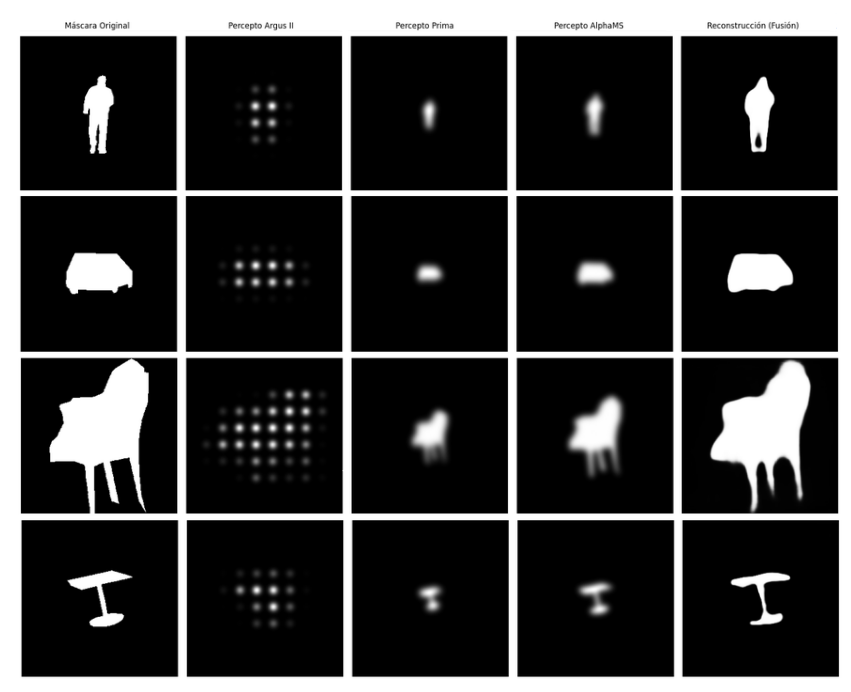
\includegraphics[width=\columnwidth]{figs/reconstrucciones_unet_fusion.png}
    \caption{Ejemplos cualitativos de reconstrucción usando U-Net de fusión. Cada fila muestra percepto, reconstrucción y máscara original.}
    \label{fig:reconstrucciones}
\end{figure}


\section{Discusión}

Los resultados muestran una diferencia clara entre las tareas de clasificación y reconstrucción. En clasificación, como se observa en el Cuadro~\ref{tab:clasificacion} y en la Fig.~\ref{fig:confusion_knn}, los desempeños fueron moderados, con un máximo de 0.611 de accuracy. Esto indica que los perceptos contienen información semántica, pero que distinguir entre clases a partir de señales degradadas sigue siendo difícil. En particular, clases con estructuras finas o alta variabilidad, como \textit{chair}, resultaron más problemáticas.

En reconstrucción, en cambio, los resultados fueron considerablemente más altos. Como muestra el Cuadro~\ref{tab:reconstruccion}, la U-Net de fusión obtuvo un Dice superior a 0.90. Además, las curvas de la Fig.~\ref{fig:curvas_recon} y los ejemplos cualitativos de la Fig.~\ref{fig:reconstrucciones} muestran que el modelo logra recuperar la forma global de los objetos. Este resultado es importante porque sugiere que, aunque el percepto no sea fácilmente interpretable como imagen natural, todavía contiene estructura espacial explotable por modelos de aprendizaje automático.

Cabe notar que los valores altos de reconstrucción deben interpretarse en el contexto del tipo de dato utilizado. Las máscaras binarias están representadas sobre fondo negro, por lo que una gran proporción de los píxeles corresponde al fondo. La pixel accuracy es especialmente sensible a este efecto, ya que puede aumentar aunque el modelo clasifique correctamente principalmente el fondo. Dice e IoU mitigan parcialmente este problema al enfocarse en la superposición entre la región predicha y la región objetivo, pero los resultados deben interpretarse considerando que la tarea no incluye textura, color ni fondo complejo.

La mejora observada en los modelos multi-implante también es relevante. Tanto en clasificación como en reconstrucción, la combinación de información de distintos implantes produjo los mejores resultados globales. Esto respalda la idea de que diferentes geometrías de implante preservan aspectos complementarios del objeto. Desde el punto de vista metodológico, esto permite comparar no solo modelos de aprendizaje, sino también representaciones perceptuales generadas por distintos dispositivos.

Respecto de la motivación aplicada, este trabajo puede interpretarse como una etapa previa hacia el diseño de filtros o transformaciones para visión protésica. Evaluar directamente qué filtro ayuda más a una persona usuaria de implante requeriría experimentos con sujetos, métricas perceptuales y una simulación más completa del sistema visual. En cambio, este trabajo propone una evaluación objetiva inicial: si una transformación genera perceptos desde los cuales se puede clasificar mejor el objeto o reconstruir mejor su forma, entonces dicha transformación preserva más información útil.

Bajo esta interpretación, las tareas de clasificación y reconstrucción funcionan como métricas proxy. La clasificación mide preservación semántica; la reconstrucción mide preservación espacial. Ninguna de las dos reemplaza una evaluación perceptual humana, pero ambas permiten comparar de forma controlada diferentes implantes, modelos y estrategias de representación. Por lo tanto, el trabajo sí tiene una conexión con un uso real: puede servir como base para seleccionar o descartar preprocesamientos visuales antes de evaluarlos en escenarios más costosos o realistas.

También existen limitaciones importantes. En primer lugar, se trabajó principalmente con máscaras binarias, no con escenas RGB completas. Esto reduce la complejidad del problema y permite aislar la forma del objeto, pero deja fuera información de color, textura y contexto. En segundo lugar, la simulación de la señal eléctrica fue simplificada y no modela completamente trenes temporales de estimulación. En tercer lugar, las métricas automáticas no garantizan por sí solas interpretabilidad humana. Por estos motivos, los resultados deben entenderse como una validación computacional preliminar, no como una demostración clínica.

\section{Conclusiones y Trabajo Futuro}

En este trabajo se desarrolló un pipeline para estudiar la información preservada en perceptos simulados de prótesis retinales. A partir de máscaras de objetos de COCO, se generaron perceptos para tres modelos de implante y se evaluaron tareas de clasificación y reconstrucción.

Los resultados muestran que los perceptos simulados conservan información útil, aunque degradada. En clasificación, el mejor modelo fue KNN multi-implante, lo que sugiere que la combinación de perceptos de distintos implantes aporta información complementaria. En reconstrucción, la U-Net de fusión alcanzó el mejor desempeño, con Dice de 0.9048 e IoU de 0.8756, mostrando que es posible recuperar con buena calidad la forma global del objeto.

Como trabajo futuro, se propone avanzar hacia el objetivo original del proyecto: comparar filtros o transformaciones aplicadas a imágenes antes de su simulación perceptual. El pipeline desarrollado permitiría evaluar objetivamente dichas transformaciones midiendo si mejoran la clasificación o reconstrucción posterior. En este esquema, los modelos ya entrenados funcionarían como función de evaluación fija: dado un filtro candidato, se procesarían las máscaras filtradas con pulse2percept y se mediría el impacto sobre la accuracy del clasificador o el Dice de la U-Net, sin necesidad de reentrenar los modelos.

Sin embargo, este enfoque de evaluación discreta presenta una limitación estructural: el espacio de filtros posibles es continuo e infinito, y la búsqueda manual solo permite explorar un número reducido de configuraciones sin garantía de encontrar el óptimo. Una solución más principiada sería aprender el filtro óptimo de forma automática mediante optimización end-to-end diferenciable, donde una red neuronal aprende directamente la transformación que maximiza el desempeño del clasificador o la U-Net. El obstáculo técnico central de este enfoque es que pulse2percept no es diferenciable, lo que impide propagar gradientes a través del simulador. Una vía prometedora para superar esto es entrenar primero un surrogate model diferenciable que aprenda a imitar el comportamiento de pulse2percept, y luego realizar el aprendizaje end-to-end a través de dicho surrogate. Esta dirección es explorada en trabajos recientes del área~\cite{granley2022}.

También se podría extender el enfoque a imágenes RGB, escenas completas, secuencias de video, segmentación semántica, métricas perceptuales y eventualmente estudios con usuarios o sujetos bajo visión protésica simulada. Otra extensión relevante sería incorporar modelos temporales de estimulación, ya que trabajos recientes muestran que los patrones espaciales y temporales de activación pueden afectar el desempeño perceptual en visión protésica simulada~\cite{kasowski2025}.


\bibliographystyle{IEEEtran}
\begin{thebibliography}{1}

\bibitem{beyeler2017}
M. Beyeler, G. M. Boynton, I. Fine, and A. Rokem, ``pulse2percept: A Python-Based Simulation Framework for Bionic Vision,'' in \emph{Proceedings of the 16th Python in Science Conference (SciPy)}, pp. 81--88, 2017.

\bibitem{han2021}
N. Han, S. Srivastava, A. Xu, D. Klein, and M. Beyeler, ``Deep Learning-Based Scene Simplification for Bionic Vision,'' arXiv:2102.00297, 2021.

\bibitem{sanchezgarcia2018}
M. Sanchez-Garcia, R. Martinez-Cantin, and J. J. Guerrero, ``Semantic and structural image segmentation for prosthetic vision,'' arXiv:1809.09607, 2018.

\bibitem{kasowski2025}
J. M. Kasowski and M. Beyeler, ``Simulated prosthetic vision identifies checkerboard as an effective raster pattern for retinal implants,'' arXiv:2501.02084, 2025.

\bibitem{kasowskietal2025}
J. M. Kasowski, A. Varshney and M. Beyeler, ``Static or Temporal? Semantic Scene Simplification to Aid Wayfinding in Immersive Simulations of Bionic Vision,'' arXiv:2507.10813, 2025.

\bibitem{granley2022}
J. Granley and M. Beyeler, ``A Deep Learning-based in silico Framework for Optimization on Retinal Prosthetic Stimulation,''  \textit{arXiv:2209.01216}, 2022.

\bibitem{coco}
T.-Y. Lin et al., ``Microsoft COCO: Common Objects in Context,'' arXiv:1405.0312, 2014.

\end{thebibliography}

\end{document}